%Description du code, du fonctionnement du moteur de simulation, des générateurs aléatoires. Ceci peut être aidé par le placement de commentaires pertinents dans le code.

%Manuel utilisateur : description du fonctionnement, paramétrage.

%Le code source, fichiers de données et exécutables seront fournis sous forme électronique dans des sous-répertoires src, data, bin respectivement. 

Le système est composé de deux parties : un programme, écrit en Java,  qui implémente la boucle de simulation, et un ficher Excel qui contient les données issues du programme et qui les traite pour en ressortir des résultats statistiques.
\\
Le programme Java implémente une boucle de simulation événementielle, telle que décrite par la figure~\ref{replique}, dans la classe principale Aéroport. 
Le processus d'initialisation remplit un agenda (de type <Events>SortedList) qui contient les événements d'arrivées d'avions dans l'espace aérien de l'aéroport, ainsi que les changement de météo. Ces événement sont générés par une boucle. 
Les intervalles de temps entre les événements dépendent de la date de l’événement précédent. Ceci est fait pour respecter le cahier des charges. 
Nous avons fait le choix de générer tout les événements d'arrivées d'avions et de changement de météo avant le parcours de la boucle principale de simulation. L'initialisation instancie également les objets représentant les infrastructures (de type Facilities), les avions étant générés durant la simulation par le traitement de l’événement correspondant à leur arrivée.
Tous les événements sont des sous-classes de la classe abstraite Events. Chacun contient sa propre méthode \textit{doSomething()} qui est appelée par la boucle de simulation. Cette méthode crée les événements dont découle l’événement courant et renvoie une chaîne de caractère décrivant l’événement qui sera intégrée dans le logger, le fichier retourné par le programme.
L'architecture du programme Java est décrite dans le diagramme de classe~\ref{class_diagramm}.
 \begin{figure}[h]
 \centering
 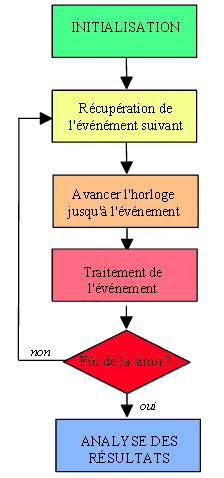
\includegraphics[scale=0.32]{replique_simu.png}
   \caption{\label{replique} Boucle de simulation}
 \end{figure}
\clearpage

\begin{figure}[h!]
\hspace{-2cm}
 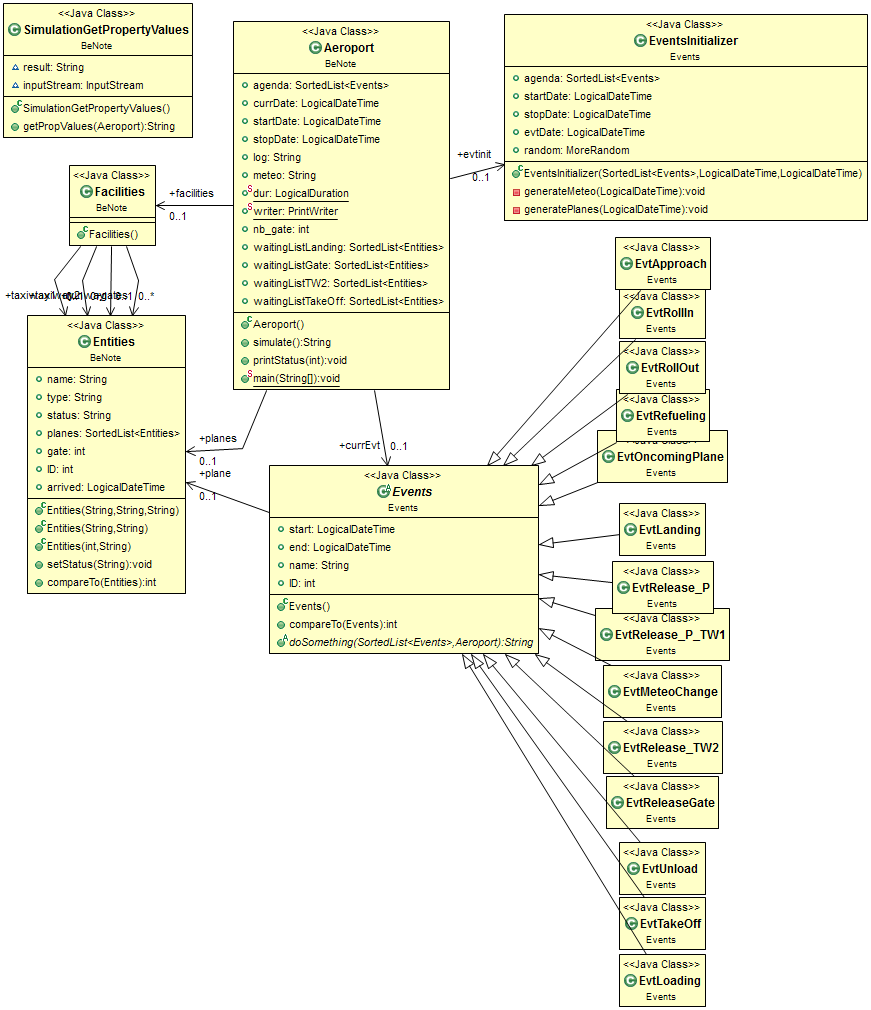
\includegraphics[scale=0.6]{Class_Diagramm.png}
  \caption{\label{class_diagramm} Diagramme de classe} 
 \end{figure}
 
